\documentclass[]{myHOWTO-V001}

\usepackage{myTCB-V001}

\title{The \textbf{myREF-V001} Package}
\version{1.00}
\author{Norbert EHART (norbert@ehart.net)}
\date{\today}

\begin{document}

\selectlanguage{english}

\maketitle
\tableofcontents

\section{Introduction}

Latex is heavily used in scientific fields, such as electrical engineering, mechanical engineering, and computer science. Especially in these areas it is almost always necessary to provide a literature reference.

Referencing is an important part of academic work. It puts your work in context, demonstrates the breadth and depth of your research, and acknowledges other people’s work. You should reference whenever you use someone else’s idea. \cite[][]{RefExplained2023}

Whenever you use an idea from someone else's work, for example from a journal article, textbook or website, you should cite the original author to make it clear where that idea came from. This is the case regardless of whether you have paraphrased, summarised or directly quoted their work. This is a key part of good practice in academic writing. \cite[][]{RefExplained2023}

This document is not intended to explain how to correctly cite, but to give a brief explanation of how \emph{the myREF-V001 package} in \LaTeX{} can be used for this purpose.

\section{Usage}

To load the package, write \Verb|\usepackage{myREF-V001}| in the preamble of your document. To use this package, it is highly recommended to have the complete \LaTeX{} distribution installed. This will avoid problems with dependencies.

\begin{mySTY}{}
[...]

\usepackage{myREF-V001}

[...]
\end{mySTY}

The first thing that should be perhaps mentioned is that a file called \emph{references.bib} has to exist in the current working directory. The contents of this file might look something like the following example.

\begin{mySTY}{}
[...]

@book{JunMXseries2012,
	author = {{Douglas Richard Hanks and Harry Reynolds}},
	title = {{Juniper MX Series}},
	date = {2012},
	publisher = {OReilly Media, Inc.},
	keywords={books},
}

@misc{BasicINT2023,
	howpublished = {\url{https://www.vivaxsolutions.com/maths/albscintgrtn.aspx}},
	keywords={online},
}

@misc{Overleaf-styBIB2023,
	howpublished = {\url{https://de.overleaf.com/learn/latex/Bibtex_bibliography_styles}},
	keywords={online},
}

[...]
\end{mySTY}

It contains the complete bibliography. Quotations in the middle of the text, works as usual

\begin{myTEXEX}{listing and text}
\lipsum[4] \cite{Overleaf-styBIB2023}	
\end{myTEXEX}

Before the reference list can be used, a \emph{bbl} file from the \emph{bib} file must be created. With \TeX studio, this can be done using the menu item \Verb|[Tools -> Bibliography]|.

\quad
\begin{myFIG}{}
	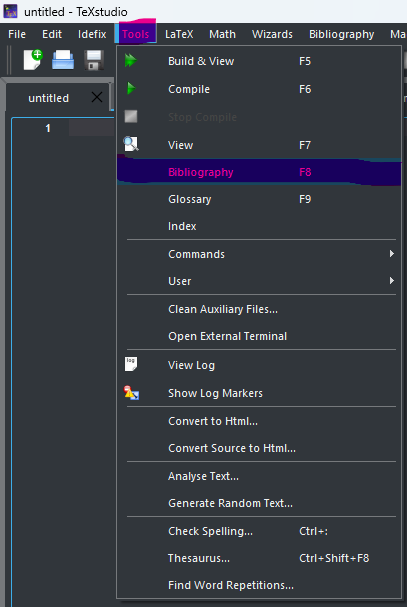
\includegraphics[width=6cm]{pictures/TeXstudio_bibliography.png}
\end{myFIG}

This process needs to be repeated every time a change is made to the bib file. Finally, the reference list can be printed in two different ways (see Example 1 and 2).

\section{Example 1}

All entries created in the \emph{bib} file are listed here. The heading is numbered and can also be found in the table of contents.

\begin{myTEXEX}{text only}
\begin{mySTY}{boxsep=0mm}
\clearpage
\pagestyle{empty}
\printbibliography[heading=bibnumbered]
\clearpage
\pagestyle{plain}
\end{mySTY}

\tcblower

\begin{center}
	\begin{myFIG}{}
		\includegraphics[page=4, scale=0.35]{examples/example01.pdf}
	\end{myFIG}
\end{center}
\end{myTEXEX}

\section{Example 2}

All entries created in the \emph{bib} file are listed here, but separated from each other. The separation can be done with the option \emph{keyword}. Every sub reference list can be given its own heading with the option \emph{title}. This heading is found as a level 2 entry, because of the option \emph{heading=subbibliography}, in the table of contents. The parent heading (level 1) must be made manually with the \emph{section} command.

\begin{myTEXEX}{text only}
\begin{mySTY}{boxsep=0mm}
\clearpage
\pagestyle{empty}
\section{References}
\printbibliography[heading=subbibliography,keyword={books},title={Books}]
\printbibliography[heading=subbibliography,keyword={online},title={Web Publications}]
\clearpage
\pagestyle{plain}
\end{mySTY}

\tcblower

\begin{center}
	\begin{myFIG}{}
		\includegraphics[page=2, scale=0.35]{examples/example01.pdf}
	\end{myFIG}
\end{center}
\end{myTEXEX}

\clearpage
\pagestyle{empty}
\printbibliography[heading=bibnumbered]
\clearpage
\pagestyle{plain}

\end{document}